\tikzsetnextfilename{ANCF_2D}
%\tikzset{external/export next=false}
\begin{figure}
	\centering
	\begin{tikzpicture}
	\node[inner sep=0pt] at (0,0)
	{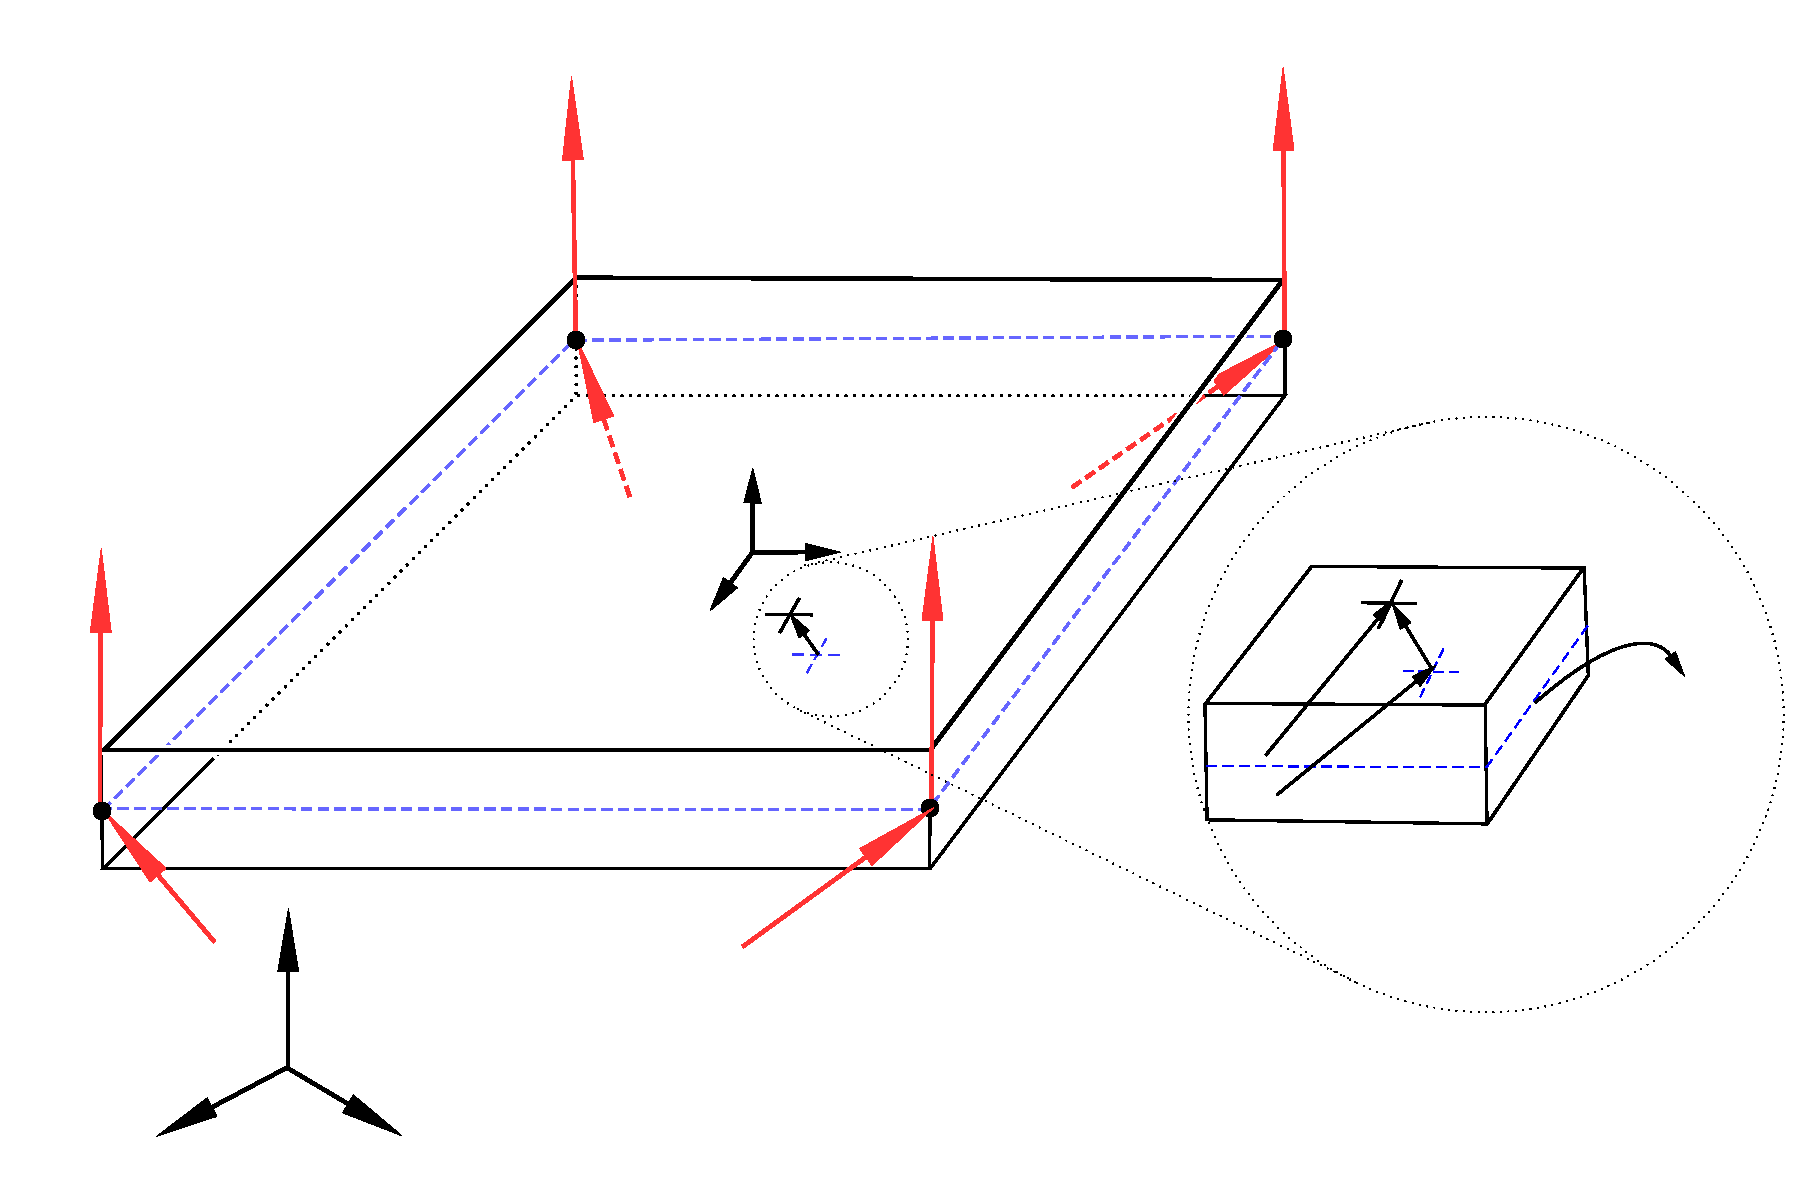
\includegraphics[width=1\textwidth]{images/2dancf.pdf}};
	\node at (-6.8,-3) {\LARGE $\mathbf{r}^1$};
	\node at (-0.5,-2.8) {\LARGE $\mathbf{r}^2$};
	\node at (2,1.8) {\LARGE $\mathbf{r}^3$};
	\node at (-2.2,1.4) {\LARGE $\mathbf{r}^4$};
	
\node at (-7.8,-0) {\LARGE $\frac{\partial\mathbf{r}^1}{\partial z}$};
\node at (0.7,-0) {\LARGE $\frac{\partial\mathbf{r}^2}{\partial z}$};
\node at (4,4.5) {\LARGE $\frac{\partial\mathbf{r}^3}{\partial z}$};
\node at (-3.5,4.5) {\LARGE $\frac{\partial\mathbf{r}^4}{\partial z}$};		
	
	
	\node at (-0.6,0.8) {\large $x$};
	\node at (-1.8,0.2) {\large $y$};
	\node at (-1.15,1.2) {\large $z$};
	
	\node at (-4.8,-5.1) {\large $X$};
	\node at (-6.5,-5.1) {\large $Y$};
	\node at (-5.3,-3.1) {\large $Z$};


\node at (3.75,-0.7)[rotate=52] {$\mathbf{r}\;(x,y,z)$};
\node at (5,-0.2) {\large $z \frac{ \partial \mathbf{r} } {\partial z} $ };
\node at (4.1,-1.5)[rotate=40] { $\mathbf{r}_m(x,y)$};
\node at (7.2,-0.8) {\large Mid-plane};
	
	
	\end{tikzpicture}
	\caption{ANCF cable element's schematic. Each node features a global position vector and a position vector gradient along the axis of the element (6DOF). Using shape functions and knowing $\xi$ one can interpolate the degrees of freedom to any point $P$ within the element. } \label{fig:ANCFCable}
\end{figure}
